% !TEX TS-program = XeLaTeX
% !TEX program = XeLaTeX
%\errorcontextlines 10000

% this is not standalone
% this is latexmlAlts to test if we need alternative latexml commands

\documentclass[10pt]{book}

\usepackage[marginparwidth=150pt]{geometry}
\usepackage{amsmath}
\usepackage{booktabs}
\usepackage{tikz}
\usepackage{enumitem}
\usepackage{latexml}
\usepackage{hyperref}

\renewcommand{\chapterautorefname}{Chap\-ter} % the default is lowercase
\renewcommand{\sectionautorefname}{Sec\-tion} % the default is lowercase
\renewcommand{\figureautorefname}{Fig\-ure} % the default is missing hyphenation
\renewcommand{\appendixname}{Ap\-pen\-di\-ces} % the default is missing hyphenation

\begin{document}

\framebox[.14\linewidth][l]{\parbox{1pt}{Chapter\\\chapterautorefname}}
\framebox[.14\linewidth][l]{\parbox{1pt}{Section\\\sectionautorefname}}
\framebox[.14\linewidth][l]{\parbox{1pt}{Figure\\\figureautorefname}}
\framebox[.14\linewidth][l]{\parbox{1pt}{Appendices\\\appendixname}}
\framebox[.14\linewidth][l]{\parbox{1pt}{150.0pt\\\the\marginparwidth}}
\framebox[.14\linewidth][l]{\parbox{1pt}{5.0pt\\\the\defaultaddspace}}

% todo tikz matrix spacing see https://github.com/brucemiller/LaTeXML/issues/794
\noindent before\\
\begin{tikzpicture}
  \matrix {
    & \node (A) {A}; \\
    \node{B};&& \node(C){C}; \\
  };
  \draw (A.south) -- (A|- C.south);
\end{tikzpicture}\\
after

Compare: % see 09_Parametric_Equations.tex
\[
\begin{gathered}\text{Choose}\\t\end{gathered}\quad
\tikz[>=latex,baseline=(current bounding box.center)]{\draw[->](0,.3)--(1,.6);\draw[->](0,-.3)--(1,-.6);}\quad
\begin{gathered}
\text{Use a function}\\f\text{ to find }x\\\bigl(x=f(t)\bigr)\\\\
\text{Use a function}\\g\text{ to find }y\\\bigl(y=g(t)\bigr)
\end{gathered}\quad
\tikz[>=latex,baseline=(current bounding box.center)]{\draw[->](0,.6)--(1,.3);\draw[->](0,-.6)--(1,-.3);}\quad
\begin{gathered}\text{Plot point}\\(x,y)\end{gathered}
\]
to:
\[
\begin{gathered}\text{Choose}\\t\end{gathered}\quad
\begin{gathered}\scalebox{3}[1]{$\nearrow$}\\\\\scalebox{3}[1]{$\searrow$}\end{gathered}\quad
\begin{gathered}
\text{Use a function}\\f\text{ to find }x\\\bigl(x=f(t)\bigr)\\\\
\text{Use a function}\\g\text{ to find }y\\\bigl(y=g(t)\bigr)
\end{gathered}\quad
\begin{gathered}\scalebox{3}[1]{$\searrow$}\\\\\scalebox{3}[1]{$\nearrow$}\end{gathered}\quad
\begin{gathered}\text{Plot point}\\(x,y)\end{gathered}
\]
to:
\begin{center}
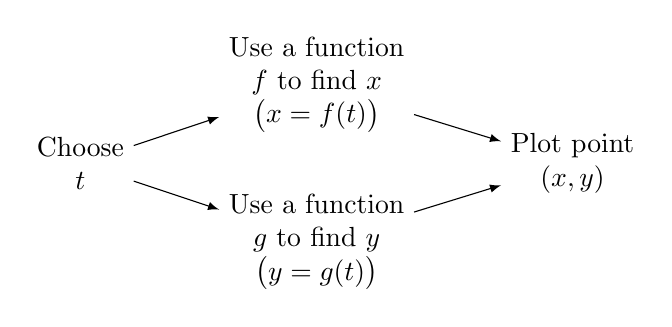
\begin{tikzpicture}[>=latex]
\draw (0,0) node (A) [align=center] {Choose \\$t$} 
      (3,1) node[align=center] (B1) {Use a function\\ $f$ to find $x$\\$\bigl(x=f(t)\bigr)$}
			(3,-1) node[align=center] (B2) {Use a function\\ $g$ to find $y$\\$\bigl(y=g(t)\bigr)$}
			(6.25,0) node [align=center] (C) {Plot point \\ $(x,y)$};
\draw [->](A) --(B1);
\draw [->](A) --(B2);
\draw [->](B1) -- (C);
\draw [->](B2) -- (C);
\end{tikzpicture}
\end{center}

\setlist[enumerate,1]{label=((\arabic*.))}
\setlist[enumerate,2]{label=((\alph*))}

\begin{enumerate}
\item problem should be ((1.)) Has parts:
\begin{enumerate}
\item should be ((a))
\item should be ((b))
\end{enumerate}
\item problem should be ((2.))
\end{enumerate}

\end{document}
